\documentclass[11pt]{article}

\newcommand{\titrechapitre}{Probabilités -- Exercices}
\newcommand{\titreclasse}{Lycée Jean-Baptiste \textsc{Corot}}
\newcommand{\pagination}{\thepage}%/\pageref{LastPage}}
\newcommand{\topbotmargins}{2cm}
%%%%%%%%%%%%%%%%%%%%%%%%%%%%%%%%%%%%%%%%%%%%%%%%%%%%%%%%%%%%%%%%%%%%%%%%%%%%%%%%
%
% PACKAGES
% ========
%
%%%%%%%%%%%%%%%%%%%%%%%%%%%%%%%%%%%%%%%%%%%%%%%%%%%%%%%%%%%%%%%%%%%%%%%%%%%%%%%%

\usepackage[english, french]{babel}
\usepackage[utf8]{inputenc}
\usepackage[T1]{fontenc}
\usepackage{graphicx}
\usepackage{amsmath,amssymb,amsthm,amsopn}
\usepackage{hyperref}

% Pour avoir l'écriture \mathscr (math script)
% ============================================

\usepackage{mathrsfs}

% Deal with coma as a decimal separator
% =====================================

\usepackage{icomma}

% Package Geometry
% ================

\usepackage[a4paper, lmargin=2cm, rmargin=2cm, top=\topbotmargins, bottom=\topbotmargins]{geometry}

% Package multicol
% ================

\usepackage{multicol}

% Redefine abstract
% =================

% Note
% ====
%
% Le reste a été commenté pour ne pas charger trop de choses au démarrage. On
% verra si on en a besoin plus tard.
%
% --------
%
%\usepackage{mathrsfs}
%\usepackage{multirow}
%\usepackage{bm}
%\hypersetup{
%    colorlinks=true,
%    linkcolor=blue,
%    citecolor=red,
%}
%\usepackage{diagbox}
%
%\usepackage{algorithm}
%\usepackage{algpseudocode}
%
%\renewcommand{\algorithmicrequire}{\textbf{Input:}}
%\renewcommand{\algorithmicensure}{\textbf{Output:}}


%%%%%%%%%%%%%%%%%%%%%%%%%%%%%%%%%%%%%%%%%%%%%%%%%%%%%%%%%%%%%%%%%%%%%%%%%%%%%%%%
%
% TIKZ
% ====
%
%%%%%%%%%%%%%%%%%%%%%%%%%%%%%%%%%%%%%%%%%%%%%%%%%%%%%%%%%%%%%%%%%%%%%%%%%%%%%%%%

\usepackage{tikz}
\usetikzlibrary{arrows}

\usepackage{tkz-tab} % Variation tables

\usepackage{pgfplots}
%\usepackage{pgf-pie} % Pie charts

\pgfplotsset{
%\newcommand{\settingsgraph}{
x=.5cm,y=.5cm,
xticklabel style = {font=\scriptsize, yshift=.1cm},
yticklabel style = {font=\scriptsize, xshift=.1cm},
axis lines=middle,
ymajorgrids=true,
xmajorgrids=true,
major grid style = {color=white!80!blue},
xmin=-5.5,
xmax=5.5,
ymin=-5.5,
ymax=5.5,
xtick={-5.0,-4.0,...,5.0},
ytick={-5.0,-4.0,...,5.0},
}

% Tikz style

\tikzset{round/.style={circle, draw=black, very thick, scale = 0.7}}
\tikzset{arrow/.style={->, >=latex}}
\tikzset{dashed-arrow/.style={->, >=latex, dashed}}

\newcommand{\point}[3]{\draw[very thick, #3] (#1-.1, #2)--(#1+.1, #2)
(#1, #2-.1)--(#1, #2+.1)}

%%%%%%%%%%%%%%%%%%%%%%%%%%%%%%%%%%%%%%%%%%%%%%%%%%%%%%%%%%%%%%%%%%%%%%%%%%%%%%%%
%
% FANCY HEADER
% ============
%
%%%%%%%%%%%%%%%%%%%%%%%%%%%%%%%%%%%%%%%%%%%%%%%%%%%%%%%%%%%%%%%%%%%%%%%%%%%%%%%%


\usepackage{fancyhdr}
\usepackage{lastpage}

\pagestyle{fancy}
\newcommand{\changefont}{\fontsize{9}{9}\selectfont}
\renewcommand{\headrulewidth}{0mm}
\renewcommand{\footrulewidth}{0mm}

\fancyhead[C]{}
\fancyhead[L]{\titreclasse}
\fancyhead[R]{\titrechapitre}
\fancyfoot[C]{}
\fancyfoot[L]{}
\fancyfoot[R]{\pagination}
\addtolength{\skip\footins}{20pt} % distance between text and footnotes

%%%%%%%%%%%%%%%%%%%%%%%%%%%%%%%%%%%%%%%%%%%%%%%%%%%%%%%%%%%%%%%%%%%%%%%%%%%%%%%%
%
% THEOREM STYLE
% =============
%
%%%%%%%%%%%%%%%%%%%%%%%%%%%%%%%%%%%%%%%%%%%%%%%%%%%%%%%%%%%%%%%%%%%%%%%%%%%%%%%%

\usepackage[tikz]{bclogo}
\usepackage{mdframed}

\usepackage{tcolorbox}
\tcbuselibrary{listings, breakable, theorems, skins}

%\newtheoremstyle{break}%
%{}{}%
%{\itshape}{}%
%{\bfseries}{}%  % Note that final punctuation is omitted.
%{\newline}{}

\newtheoremstyle{scbf}%
{}{}%
{}{}%
%{\scshape}{}%  % Note that final punctuation is omitted.
{\bfseries\scshape}{}%  % Note that final punctuation is omitted.
{\newline}{}

%\theoremstyle{break}
%\theoremstyle{plain}
%\newtheorem{thm}{Theorem}[section]
%\newtheorem{lm}[thm]{Lemma}
%\newtheorem{prop}[thm]{Proposition}
%\newtheorem{cor}[thm]{Corollary}

%\theoremstyle{scbf}
%\newtheorem{exo}{$\star$ Exercice}

%\theoremstyle{definition}
%\newtheorem{defi}[thm]{Definition}
%\newtheorem{ex}[thm]{Example}

%\theoremstyle{remark}
%\newtheorem{rem}[thm]{Remark}

% Defining the Remark environment
% ===============================

\newenvironment{rmq}
  {
    \begin{bclogo}[logo=\bcinfo, noborder=true]{Remarque}
  }
  {
    \end{bclogo}
  }

% Defining the exercise environment
% =================================

\newcounter{exos}
\setcounter{exos}{1}

\newenvironment{exo}
  {
    \begin{bclogo}[logo=\bccrayon, noborder=true]{Exercice \theexos}
  }
  {
    \end{bclogo}
    \addtocounter{exos}{1}
  }


% Redefining the proof environment from amsthm
% ============================================

\tcolorboxenvironment{proof}{
  blanker, breakable, before skip=10pt,after skip=10pt,
  borderline west={1mm}{0pt}{red},
  left=5mm,
}

% Defining the definition environment
% ===================================

\colorlet{coldef}{black!50!green}

\newcounter{defis}
\setcounter{defis}{1}

\newenvironment{defi}[1]
  {
    \begin{defihid}{{#1}}{\thedefis}
  }
  {
    \end{defihid}
    \addtocounter{defis}{1}
  }

\newtcolorbox{defihid}[2]{%
  empty,title={ {\bfseries Définition {#2}} ({#1})},attach boxed title to top left,
boxed title style={empty,size=minimal,toprule=2pt,top=4pt,
overlay={\draw[coldef,line width=2pt]
([yshift=-1pt]frame.north west)--([yshift=-1pt]frame.north east);}},
coltitle=coldef,
before=\par\medskip\noindent,parbox=false,boxsep=0pt,left=0pt,right=3mm,top=4pt,
breakable,pad at break*=0mm,vfill before first,
overlay unbroken={\draw[coldef,line width=1pt]
([yshift=-1pt]title.north east)--([xshift=-0.5pt,yshift=-1pt]title.north-|frame.east)
--([xshift=-0.5pt]frame.south east)--(frame.south west); },
overlay first={\draw[coldef,line width=1pt]
([yshift=-1pt]title.north east)--([xshift=-0.5pt,yshift=-1pt]title.north-|frame.east)
--([xshift=-0.5pt]frame.south east); },
overlay middle={\draw[coldef,line width=1pt] ([xshift=-0.5pt]frame.north east)
--([xshift=-0.5pt]frame.south east); },
overlay last={\draw[coldef,line width=1pt] ([xshift=-0.5pt]frame.north east)
--([xshift=-0.5pt]frame.south east)--(frame.south west);},%
}

\newenvironment{notation}
  {
    \begin{notationhid}{\thedefis}
  }
  {
    \end{notationhid}
    \addtocounter{defis}{1}
  }

\newtcolorbox{notationhid}[1]{%
  empty,title={Notation {#1}},attach boxed title to top left,
boxed title style={empty,size=minimal,toprule=2pt,top=4pt,
overlay={\draw[coldef,line width=2pt]
([yshift=-1pt]frame.north west)--([yshift=-1pt]frame.north east);}},
coltitle=coldef,fonttitle=\bfseries,
before=\par\medskip\noindent,parbox=false,boxsep=0pt,left=0pt,right=3mm,top=4pt,
breakable,pad at break*=0mm,vfill before first,
overlay unbroken={\draw[coldef,line width=1pt]
([yshift=-1pt]title.north east)--([xshift=-0.5pt,yshift=-1pt]title.north-|frame.east)
--([xshift=-0.5pt]frame.south east)--(frame.south west); },
overlay first={\draw[coldef,line width=1pt]
([yshift=-1pt]title.north east)--([xshift=-0.5pt,yshift=-1pt]title.north-|frame.east)
--([xshift=-0.5pt]frame.south east); },
overlay middle={\draw[coldef,line width=1pt] ([xshift=-0.5pt]frame.north east)
--([xshift=-0.5pt]frame.south east); },
overlay last={\draw[coldef,line width=1pt] ([xshift=-0.5pt]frame.north east)
--([xshift=-0.5pt]frame.south east)--(frame.south west);},%
}


% Defining the proposition, theorem, etc. environment
% ===================================================

\colorlet{colprop}{red!75!black}

\newcounter{props}
\setcounter{props}{1}

\newenvironment{prop}
  {
    \begin{prophid}{\theprops}
  }
  {
    \end{prophid}
    \refstepcounter{props}
  }

\newtcolorbox{prophid}[1]{%
empty,title={Propriété {#1}},attach boxed title to top left,
boxed title style={empty,size=minimal,toprule=2pt,top=4pt,
overlay={\draw[colprop,line width=2pt]
([yshift=-1pt]frame.north west)--([yshift=-1pt]frame.north east);}},
coltitle=colprop,fonttitle=\bfseries,
before=\par\medskip\noindent,parbox=false,boxsep=0pt,left=0pt,right=3mm,top=4pt,
breakable,pad at break*=0mm,vfill before first,
overlay unbroken={\draw[colprop,line width=1pt]
([yshift=-1pt]title.north east)--([xshift=-0.5pt,yshift=-1pt]title.north-|frame.east)
--([xshift=-0.5pt]frame.south east)--(frame.south west); },
overlay first={\draw[colprop,line width=1pt]
([yshift=-1pt]title.north east)--([xshift=-0.5pt,yshift=-1pt]title.north-|frame.east)
--([xshift=-0.5pt]frame.south east); },
overlay middle={\draw[colprop,line width=1pt] ([xshift=-0.5pt]frame.north east)
--([xshift=-0.5pt]frame.south east); },
overlay last={\draw[colprop,line width=1pt] ([xshift=-0.5pt]frame.north east)
--([xshift=-0.5pt]frame.south east)--(frame.south west);},%
}

\newenvironment{propadm}
  {
    \begin{propadmhid}{\theprops}
  }
  {
    \end{propadmhid}
    \refstepcounter{props}
  }

  \newtcolorbox{propadmhid}[1]{%
    empty,title={{\bfseries Propriété {#1}} (admise)},attach boxed title to top left,
boxed title style={empty,size=minimal,toprule=2pt,top=4pt,
overlay={\draw[colprop,line width=2pt]
([yshift=-1pt]frame.north west)--([yshift=-1pt]frame.north east);}},
coltitle=colprop,%fonttitle=\bfseries,
before=\par\medskip\noindent,parbox=false,boxsep=0pt,left=0pt,right=3mm,top=4pt,
breakable,pad at break*=0mm,vfill before first,
overlay unbroken={\draw[colprop,line width=1pt]
([yshift=-1pt]title.north east)--([xshift=-0.5pt,yshift=-1pt]title.north-|frame.east)
--([xshift=-0.5pt]frame.south east)--(frame.south west); },
overlay first={\draw[colprop,line width=1pt]
([yshift=-1pt]title.north east)--([xshift=-0.5pt,yshift=-1pt]title.north-|frame.east)
--([xshift=-0.5pt]frame.south east); },
overlay middle={\draw[colprop,line width=1pt] ([xshift=-0.5pt]frame.north east)
--([xshift=-0.5pt]frame.south east); },
overlay last={\draw[colprop,line width=1pt] ([xshift=-0.5pt]frame.north east)
--([xshift=-0.5pt]frame.south east)--(frame.south west);},%
}

\newenvironment{propnom}[1]
  {
    \begin{propnomhid}{#1}{\theprops}
  }
  {
    \end{propnomhid}
    \refstepcounter{props}
  }

\newtcolorbox{propnomhid}[2]{%
empty,title={{\bfseries Propriété {#2}} ({#1})},attach boxed title to top left,
boxed title style={empty,size=minimal,toprule=2pt,top=4pt,
overlay={\draw[colprop,line width=2pt]
([yshift=-1pt]frame.north west)--([yshift=-1pt]frame.north east);}},
coltitle=colprop,
before=\par\medskip\noindent,parbox=false,boxsep=0pt,left=0pt,right=3mm,top=4pt,
breakable,pad at break*=0mm,vfill before first,
overlay unbroken={\draw[colprop,line width=1pt]
([yshift=-1pt]title.north east)--([xshift=-0.5pt,yshift=-1pt]title.north-|frame.east)
--([xshift=-0.5pt]frame.south east)--(frame.south west); },
overlay first={\draw[colprop,line width=1pt]
([yshift=-1pt]title.north east)--([xshift=-0.5pt,yshift=-1pt]title.north-|frame.east)
--([xshift=-0.5pt]frame.south east); },
overlay middle={\draw[colprop,line width=1pt] ([xshift=-0.5pt]frame.north east)
--([xshift=-0.5pt]frame.south east); },
overlay last={\draw[colprop,line width=1pt] ([xshift=-0.5pt]frame.north east)
--([xshift=-0.5pt]frame.south east)--(frame.south west);},%
}




\newenvironment{thm}
  {
    \begin{thmhid}{\theprops}
  }
  {
    \end{thmhid}
    \refstepcounter{props}
  }

\newtcolorbox{thmhid}[1]{%
empty,title={Théorème {#1}},attach boxed title to top left,
boxed title style={empty,size=minimal,toprule=2pt,top=4pt,
overlay={\draw[colprop,line width=2pt]
([yshift=-1pt]frame.north west)--([yshift=-1pt]frame.north east);}},
coltitle=colprop,fonttitle=\bfseries,
before=\par\medskip\noindent,parbox=false,boxsep=0pt,left=0pt,right=3mm,top=4pt,
breakable,pad at break*=0mm,vfill before first,
overlay unbroken={\draw[colprop,line width=1pt]
([yshift=-1pt]title.north east)--([xshift=-0.5pt,yshift=-1pt]title.north-|frame.east)
--([xshift=-0.5pt]frame.south east)--(frame.south west); },
overlay first={\draw[colprop,line width=1pt]
([yshift=-1pt]title.north east)--([xshift=-0.5pt,yshift=-1pt]title.north-|frame.east)
--([xshift=-0.5pt]frame.south east); },
overlay middle={\draw[colprop,line width=1pt] ([xshift=-0.5pt]frame.north east)
--([xshift=-0.5pt]frame.south east); },
overlay last={\draw[colprop,line width=1pt] ([xshift=-0.5pt]frame.north east)
--([xshift=-0.5pt]frame.south east)--(frame.south west);},%
}

\newenvironment{thmadm}
  {
    \begin{thmadmhid}{\theprops}
  }
  {
    \end{thmadmhid}
    \refstepcounter{props}
  }

  \newtcolorbox{thmadmhid}[1]{%
    empty,title={{\bfseries Théorème {#1}} (admis)},attach boxed title to top left,
boxed title style={empty,size=minimal,toprule=2pt,top=4pt,
overlay={\draw[colprop,line width=2pt]
([yshift=-1pt]frame.north west)--([yshift=-1pt]frame.north east);}},
coltitle=colprop,%fonttitle=\bfseries,
before=\par\medskip\noindent,parbox=false,boxsep=0pt,left=0pt,right=3mm,top=4pt,
breakable,pad at break*=0mm,vfill before first,
overlay unbroken={\draw[colprop,line width=1pt]
([yshift=-1pt]title.north east)--([xshift=-0.5pt,yshift=-1pt]title.north-|frame.east)
--([xshift=-0.5pt]frame.south east)--(frame.south west); },
overlay first={\draw[colprop,line width=1pt]
([yshift=-1pt]title.north east)--([xshift=-0.5pt,yshift=-1pt]title.north-|frame.east)
--([xshift=-0.5pt]frame.south east); },
overlay middle={\draw[colprop,line width=1pt] ([xshift=-0.5pt]frame.north east)
--([xshift=-0.5pt]frame.south east); },
overlay last={\draw[colprop,line width=1pt] ([xshift=-0.5pt]frame.north east)
--([xshift=-0.5pt]frame.south east)--(frame.south west);},%
}

\newenvironment{thmnom}[1]
  {
    \begin{thmnomhid}{#1}{\theprops}
  }
  {
    \end{thmnomhid}
    \refstepcounter{props}
  }

\newtcolorbox{thmnomhid}[2]{%
empty,title={{\bfseries Théorème {#2}} ({#1})},attach boxed title to top left,
boxed title style={empty,size=minimal,toprule=2pt,top=4pt,
overlay={\draw[colprop,line width=2pt]
([yshift=-1pt]frame.north west)--([yshift=-1pt]frame.north east);}},
coltitle=colprop,
before=\par\medskip\noindent,parbox=false,boxsep=0pt,left=0pt,right=3mm,top=4pt,
breakable,pad at break*=0mm,vfill before first,
overlay unbroken={\draw[colprop,line width=1pt]
([yshift=-1pt]title.north east)--([xshift=-0.5pt,yshift=-1pt]title.north-|frame.east)
--([xshift=-0.5pt]frame.south east)--(frame.south west); },
overlay first={\draw[colprop,line width=1pt]
([yshift=-1pt]title.north east)--([xshift=-0.5pt,yshift=-1pt]title.north-|frame.east)
--([xshift=-0.5pt]frame.south east); },
overlay middle={\draw[colprop,line width=1pt] ([xshift=-0.5pt]frame.north east)
--([xshift=-0.5pt]frame.south east); },
overlay last={\draw[colprop,line width=1pt] ([xshift=-0.5pt]frame.north east)
--([xshift=-0.5pt]frame.south east)--(frame.south west);},%
}

\newenvironment{coro}
  {
    \begin{corohid}{\theprops}
  }
  {
    \end{corohid}
    \refstepcounter{props}
  }

  \newtcolorbox{corohid}[1]{%
  empty,title={Corollaire {#1}},attach boxed title to top left,
boxed title style={empty,size=minimal,toprule=2pt,top=4pt,
overlay={\draw[colprop,line width=2pt]
([yshift=-1pt]frame.north west)--([yshift=-1pt]frame.north east);}},
coltitle=colprop,fonttitle=\bfseries,
before=\par\medskip\noindent,parbox=false,boxsep=0pt,left=0pt,right=3mm,top=4pt,
breakable,pad at break*=0mm,vfill before first,
overlay unbroken={\draw[colprop,line width=1pt]
([yshift=-1pt]title.north east)--([xshift=-0.5pt,yshift=-1pt]title.north-|frame.east)
--([xshift=-0.5pt]frame.south east)--(frame.south west); },
overlay first={\draw[colprop,line width=1pt]
([yshift=-1pt]title.north east)--([xshift=-0.5pt,yshift=-1pt]title.north-|frame.east)
--([xshift=-0.5pt]frame.south east); },
overlay middle={\draw[colprop,line width=1pt] ([xshift=-0.5pt]frame.north east)
--([xshift=-0.5pt]frame.south east); },
overlay last={\draw[colprop,line width=1pt] ([xshift=-0.5pt]frame.north east)
--([xshift=-0.5pt]frame.south east)--(frame.south west);},%
}

\newenvironment{lemme}
  {
    \begin{lemmehid}{\theprops}
  }
  {
    \end{lemmehid}
    \refstepcounter{props}
  }

  \newtcolorbox{lemmehid}[1]{%
  empty,title={Lemme {#1}},attach boxed title to top left,
boxed title style={empty,size=minimal,toprule=2pt,top=4pt,
overlay={\draw[colprop,line width=2pt]
([yshift=-1pt]frame.north west)--([yshift=-1pt]frame.north east);}},
coltitle=colprop,fonttitle=\bfseries,
before=\par\medskip\noindent,parbox=false,boxsep=0pt,left=0pt,right=3mm,top=4pt,
breakable,pad at break*=0mm,vfill before first,
overlay unbroken={\draw[colprop,line width=1pt]
([yshift=-1pt]title.north east)--([xshift=-0.5pt,yshift=-1pt]title.north-|frame.east)
--([xshift=-0.5pt]frame.south east)--(frame.south west); },
overlay first={\draw[colprop,line width=1pt]
([yshift=-1pt]title.north east)--([xshift=-0.5pt,yshift=-1pt]title.north-|frame.east)
--([xshift=-0.5pt]frame.south east); },
overlay middle={\draw[colprop,line width=1pt] ([xshift=-0.5pt]frame.north east)
--([xshift=-0.5pt]frame.south east); },
overlay last={\draw[colprop,line width=1pt] ([xshift=-0.5pt]frame.north east)
--([xshift=-0.5pt]frame.south east)--(frame.south west);},%
}

\colorlet{colexemple}{blue!50!black}
%\newtcolorbox{exemple}{empty, title=Exemple, attach boxed title to top left,
%  boxed title style={empty, size=minimal, toprule=2pt, top=4pt,
%    overlay={\draw[colexemple,line width=2pt]
%([yshift=-1pt]frame.north west)--([yshift=-1pt]frame.north east);}},
%coltitle=colexemple,fonttitle=\bfseries,%\large\bfseries,
%before=\par\medskip\noindent,parbox=false,boxsep=0pt,left=0pt,right=3mm,top=4pt,
%overlay={\draw[colexemple,line width=1pt]
%([yshift=-1pt]title.north east)--([xshift=-0.5pt,yshift=-1pt]title.north-|frame.east)
%--([xshift=-0.5pt]frame.south east)--(frame.south west); },
%}

\newcounter{exemples}
\setcounter{exemples}{1}

\newenvironment{exemple}
  {
    \begin{exemplehid}{\theexemples}
  }
  {
    \end{exemplehid}
    \addtocounter{exemples}{1}
  }

\newtcolorbox{exemplehid}[1]{%
empty,title={Exemple {#1}},attach boxed title to top left,
boxed title style={empty,size=minimal,toprule=2pt,top=4pt,
overlay={\draw[colexemple,line width=2pt]
([yshift=-1pt]frame.north west)--([yshift=-1pt]frame.north east);}},
coltitle=colexemple,fonttitle=\bfseries,
before=\par\medskip\noindent,parbox=false,boxsep=0pt,left=0pt,right=3mm,top=4pt,
breakable,pad at break*=0mm,vfill before first,
overlay unbroken={\draw[colexemple,line width=1pt]
([yshift=-1pt]title.north east)--([xshift=-0.5pt,yshift=-1pt]title.north-|frame.east)
--([xshift=-0.5pt]frame.south east)--(frame.south west); },
overlay first={\draw[colexemple,line width=1pt]
([yshift=-1pt]title.north east)--([xshift=-0.5pt,yshift=-1pt]title.north-|frame.east)
--([xshift=-0.5pt]frame.south east); },
overlay middle={\draw[colexemple,line width=1pt] ([xshift=-0.5pt]frame.north east)
--([xshift=-0.5pt]frame.south east); },
overlay last={\draw[colexemple,line width=1pt] ([xshift=-0.5pt]frame.north east)
--([xshift=-0.5pt]frame.south east)--(frame.south west);},%
}

\newenvironment{contrex}
  {
    \begin{contrexhid}{\theexemples}
  }
  {
    \end{contrexhid}
    \addtocounter{exemples}{1}
  }

\newtcolorbox{contrexhid}[1]{%
empty,title={Contre-exemple {#1}},attach boxed title to top left,
boxed title style={empty,size=minimal,toprule=2pt,top=4pt,
overlay={\draw[colexemple,line width=2pt]
([yshift=-1pt]frame.north west)--([yshift=-1pt]frame.north east);}},
coltitle=colexemple,fonttitle=\bfseries,
before=\par\medskip\noindent,parbox=false,boxsep=0pt,left=0pt,right=3mm,top=4pt,
breakable,pad at break*=0mm,vfill before first,
overlay unbroken={\draw[colexemple,line width=1pt]
([yshift=-1pt]title.north east)--([xshift=-0.5pt,yshift=-1pt]title.north-|frame.east)
--([xshift=-0.5pt]frame.south east)--(frame.south west); },
overlay first={\draw[colexemple,line width=1pt]
([yshift=-1pt]title.north east)--([xshift=-0.5pt,yshift=-1pt]title.north-|frame.east)
--([xshift=-0.5pt]frame.south east); },
overlay middle={\draw[colexemple,line width=1pt] ([xshift=-0.5pt]frame.north east)
--([xshift=-0.5pt]frame.south east); },
overlay last={\draw[colexemple,line width=1pt] ([xshift=-0.5pt]frame.north east)
--([xshift=-0.5pt]frame.south east)--(frame.south west);},%
}

\newenvironment{app}
  {
    \begin{apphid}{\theexemples}
  }
  {
    \end{apphid}
    \addtocounter{exemples}{1}
  }

\newtcolorbox{apphid}[1]{%
empty,title={Application {#1}},attach boxed title to top left,
boxed title style={empty,size=minimal,toprule=2pt,top=4pt,
overlay={\draw[colexemple,line width=2pt]
([yshift=-1pt]frame.north west)--([yshift=-1pt]frame.north east);}},
coltitle=colexemple,fonttitle=\bfseries,
before=\par\medskip\noindent,parbox=false,boxsep=0pt,left=0pt,right=3mm,top=4pt,
breakable,pad at break*=0mm,vfill before first,
overlay unbroken={\draw[colexemple,line width=1pt]
([yshift=-1pt]title.north east)--([xshift=-0.5pt,yshift=-1pt]title.north-|frame.east)
--([xshift=-0.5pt]frame.south east)--(frame.south west); },
overlay first={\draw[colexemple,line width=1pt]
([yshift=-1pt]title.north east)--([xshift=-0.5pt,yshift=-1pt]title.north-|frame.east)
--([xshift=-0.5pt]frame.south east); },
overlay middle={\draw[colexemple,line width=1pt] ([xshift=-0.5pt]frame.north east)
--([xshift=-0.5pt]frame.south east); },
overlay last={\draw[colexemple,line width=1pt] ([xshift=-0.5pt]frame.north east)
--([xshift=-0.5pt]frame.south east)--(frame.south west);},%
}

%%%%%%%%%%%%%%%%%%%%%%%%%%%%%%%%%%%%%%%%%%%%%%%%%%%%%%%%%%%%%%%%%%%%%%%%%%%%%%%%
%
% ENUMERATE
% =========
%
%%%%%%%%%%%%%%%%%%%%%%%%%%%%%%%%%%%%%%%%%%%%%%%%%%%%%%%%%%%%%%%%%%%%%%%%%%%%%%%%

\usepackage{enumerate}
\usepackage{enumitem}

% To have special enumerate items like
%
% 1/
% 2/
% 3/

%%%%%%%%%%%%%%%%%%%%%%%%%%%%%%%%%%%%%%%%%%%%%%%%%%%%%%%%%%%%%%%%%%%%%%%%%%%%%%%%
%
% ARRAYS
% ======
%
%%%%%%%%%%%%%%%%%%%%%%%%%%%%%%%%%%%%%%%%%%%%%%%%%%%%%%%%%%%%%%%%%%%%%%%%%%%%%%%%


\usepackage{array}
\usepackage{makecell} % Used to break lines within arrays
\usepackage{multirow}
\usepackage{booktabs} % Used to have nice arrays with headrules

%%%%%%%%%%%%%%%%%%%%%%%%%%%%%%%%%%%%%%%%%%%%%%%%%%%%%%%%%%%%%%%%%%%%%%%%%%%%%%%%
%
% WRITE CODE
% ==========
%
%%%%%%%%%%%%%%%%%%%%%%%%%%%%%%%%%%%%%%%%%%%%%%%%%%%%%%%%%%%%%%%%%%%%%%%%%%%%%%%%

\usepackage{listings}
\usepackage{xcolor}

%New colors defined below
\definecolor{codegreen}{rgb}{0,0.6,0}
\definecolor{codegray}{rgb}{0.5,0.5,0.5}
\definecolor{codepurple}{rgb}{0.58,0,0.82}
\definecolor{backcolour}{rgb}{0.95,0.95,0.92}

%Code listing style named "mystyle"
\lstdefinestyle{python}{
  %backgroundcolor=\color{backcolour},
  commentstyle=\color{codegreen},
  keywordstyle=\color{magenta},
  numberstyle=\tiny\color{codegray},
  stringstyle=\color{codepurple},
  basicstyle=\ttfamily\footnotesize,
  breakatwhitespace=false,
  breaklines=true,
  captionpos=b,
  keepspaces=true,
  numbers=left,
  numbersep=5pt,
  showspaces=false,
  showstringspaces=false,
  showtabs=false,
  tabsize=2
}

\lstset{style=python}

%%%%%%%%%%%%%%%%%%%%%%%%%%%%%%%%%%%%%%%%%%%%%%%%%%%%%%%%%%%%%%%%%%%%%%%%%%%%%%%%
%
% Tabular 
% =======
%
%%%%%%%%%%%%%%%%%%%%%%%%%%%%%%%%%%%%%%%%%%%%%%%%%%%%%%%%%%%%%%%%%%%%%%%%%%%%%%%%

% In order to obtain a tabular with given width.

\usepackage{tabularx}
\newcolumntype{Y}{>{\centering\arraybackslash}X}
\newcolumntype{R}{>{\raggedright\arraybackslash}X}
\newcolumntype{L}{>{\raggedleft\arraybackslash}X}
% \usepackage{tabulary} % younger brother

%%%%%%%%%%%%%%%%%%%%%%%%%%%%%%%%%%%%%%%%%%%%%%%%%%%%%%%%%%%%%%%%%%%%%%%%%%%%%%%%
%
% MACROS
% ======
%
%%%%%%%%%%%%%%%%%%%%%%%%%%%%%%%%%%%%%%%%%%%%%%%%%%%%%%%%%%%%%%%%%%%%%%%%%%%%%%%%

% Math Operators

\DeclareMathOperator{\Card}{Card}
\DeclareMathOperator{\Gal}{Gal}
\DeclareMathOperator{\Id}{Id}
\DeclareMathOperator{\Img}{Im}
\DeclareMathOperator{\Ker}{Ker}
\DeclareMathOperator{\Minpoly}{Minpoly}
\DeclareMathOperator{\Mod}{mod}
\DeclareMathOperator{\Ord}{Ord}
\DeclareMathOperator{\ppcm}{ppcm}
\DeclareMathOperator{\pgcd}{pgcd}
\DeclareMathOperator{\tr}{Tr}
\DeclareMathOperator{\Vect}{Vect}
\DeclareMathOperator{\Span}{Span}
\DeclareMathOperator{\rank}{rank}
\DeclareMathOperator{\rg}{rg}
\DeclareMathOperator{\ev}{ev}
\DeclareMathOperator{\Var}{Var}

% Shortcuts

\newcommand{\eg}{\emph{e.g. }}
\newcommand{\ent}[2]{[\![#1,#2]\!]}
\newcommand{\ie}{\emph{i.e. }}
\newcommand{\ps}[2]{\left\langle#1,#2\right\rangle}
\newcommand{\eqdef}{\overset{\text{def}}{=}}
\newcommand{\E}{\mathcal{E}}
\newcommand{\M}{\mathcal{M}}
\newcommand{\A}{\mathcal{A}}
\newcommand{\B}{\mathcal{B}}
\newcommand{\R}{\mathcal{R}}
\newcommand{\D}{\mathcal{D}}
\newcommand{\Pcal}{\mathcal{P}}
\newcommand{\K}{\mathbf{k}}
\newcommand{\vect}[1]{\overrightarrow{#1}}


%\input{layout-nb.tex}

\begin{document}
%\maketitle\thispagestyle{fancy}

\begin{exo}
  Dans chacun des cas suivants, déterminer l'univers associé à l'expérience
  aléatoire décrite.
  \begin{enumerate}
    \item On lance un dé dont les faces sont numérotées de $1$ à $12$ et on
      s'intéresse au nombre obtenu.
    \item Une urne contient des jetons bleurs, rouges, verts et jaunes. On en
      tire un au hasard et on s'intéresse à sa couleur.
    \item On choisit au hasard un élève dans une classe de seconde et on veut
      savoir si c'est une fille ou un garçon.
  \end{enumerate}
\end{exo}

\begin{exo}
  Dans une maternité, sur les $640$ bébés nés cette année, $336$ sont des
  garçons. On choisit au hasard un bébé né dans cette maternité.
  \begin{enumerate}
    \item Quelle est la probabilité que ce soit un garçon ?
    \item En déduire la probabilité que ce soit une fille.
  \end{enumerate}
\end{exo}

\begin{exo}
  On pioche une carte au hasard dans un jeu de $32$ cartes et on s'intéresse à
  sa valeur.
  \begin{enumerate}
    \item Donner l'univers associé à cette expérience aléatoire.
    \item Quelle est la probabilité de tirer un as ?
    \item Quelle est la probabilité de tirer une figure (roi, dame ou valet) ?
  \end{enumerate}
\end{exo}

\begin{exo}
  On choisit au hasard un élève dans la cour du lycée. Imaginer cinq
  expériences aléatoires dont les univers sont différents.
\end{exo}

\begin{exo}
  On lance simultanément deux dés tétraédriques (à $4$ faces) dont les faces
  sont numérotées de $1$ à $4$ et on s'intéresse au produit des deux nombres
  obtenus.
  \begin{enumerate}
    \item Déterminer l'univers associé à cette expérience aléatoire.
    \item Quelle est la probabilité d'obtenir un $1$ ?
    \item Quelle est la probabilité d'obtenir un $2$ ?
    \item Quelle est la probabilité d'obtenir un $4$ ?
  \end{enumerate}
\end{exo}

\begin{exo}
  On considère un cadenas dont la clé est un code à trois chiffres. On tente une
  combinaison au hasard.
  \begin{enumerate}
    \item Combien y a-t-il de codes possibles ?
    \item En déduire la probabilité de trouver le bon code.
  \end{enumerate}
\end{exo}

\begin{exo}~\\
  \begin{minipage}[]{.5\textwidth}
    Lors d'une kermesse, dans un stand, sont disposées trois roues ci-contre.
    Tous les secteurs angulaires d'une même roue ont la même mesure. Le joueur
    doit choisir une des trois roues et la lancer. Il remporte un lot s'il tombe
    sur un secteur coloré.\\
    Quelle roue le joueur doit-il choisir ?
  \end{minipage}
  \begin{minipage}[]{.5\textwidth}
    \begin{center}
      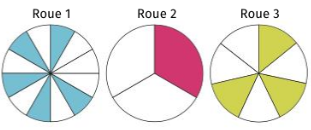
\includegraphics[scale=.7]{roues.png}
    \end{center}
  \end{minipage}
\end{exo}

\begin{exo}
  Le jeu d'échecs est composé de $16$ pièces blanches et de $16$ noires
  réparties comme suit : un roi, une dame, deux fous, deux cavaliers, deux tours
  et huit pions. Les pièces mineures le feu et le cavalier alors que les pièces
  lourdes sont la dame et la tour. On choisit une pièce au hasard parmi toutes
  les pièces du jeu. Quelle est la probabilité que ce soit :
  \begin{enumerate}
    \item un pion ?
    \item une pièce mineure ?
    \item une pièce lourde ?
  \end{enumerate}
\end{exo}

\begin{exo}
  On considère un dé icosaédrique dont les faces sont numérotées de $1$ à $20$,
  que l'on suppose bien équilibré. On lance le dé et on considère les événements
  :
  \begin{itemize}
    \item $A$ : « on obtient un nombre pair » ;
    \item $B$ : « on obtient un diviseur de $20$ » ;
    \item $C$ : « on obtient un multiple de $4$ ».
  \end{itemize}
  Écrire chaque événement sous forme d'un ensemble des issues possibles et
  calculer leur probabilité.
\end{exo}

\begin{exo}~\\
  \begin{minipage}[]{.5\textwidth}
    Dans la population mondiale, les groupes sanguins sont répartis selon le
    tableau ci-contre. Gr\^ace aux données de ce tableau, si on choisit au
    hasard une personne dans la population mondiale, quelle est la probabilité
    qu'elle soit :
  \end{minipage}
  \begin{minipage}[]{.5\textwidth}
    \begin{center}
      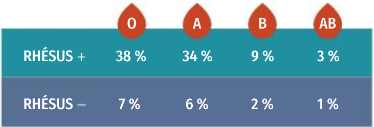
\includegraphics[scale=.6]{sang.png}
    \end{center}
  \end{minipage}
  \begin{enumerate}
    \item donneur universel, c'est-à-dire qu'elle soit du groupe O et de
        rhésus - ?
    \item du groupe AB ?
    \item de rhésus + ?
  \end{enumerate}
  \emph{On prendra soin de bien définir l'univers, la loi de probabilité, et les
  événements.}
\end{exo}

\begin{exo}~\\
  \begin{minipage}[]{.7\textwidth}
    À la bataille navale, chaque joueur a une flotte composée de cinq bateaux :
    un porte-avions ($5$ cases), un croiseur ($4$ cases), un contre-torpilleur
    ($3$ cases), un sous-marin ($3$ cases) et un torpilleur ($2$ cases). Une
    joueuse a disposé ses bateaux comme représentés ci-après. Les bateaux sont
    obligatoirement disposés horizontalement ou verticalement. L'autre joueur
    choisit de tirer sur une case au hasard.
    \begin{enumerate}
      \item Quelle est la probabilité qu'il touche un bateau ?
      \item Quelle est la probabilité qu'il touche un bateau s'il décide de ne
        tirer que dans les colonnes D et H ?
    \end{enumerate}
  \end{minipage}
  \begin{minipage}[]{.3\textwidth}
    \begin{center}
      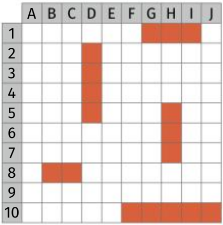
\includegraphics[scale=.5]{bataille.png}
    \end{center}
  \end{minipage}
\begin{enumerate}
    \setcounter{enumi}{2}
  \item Au tour précédent, il a touché la case D4. Quelle est la probabilité de
    toucher à nouveau le croiseur en jouant correctement ?
\end{enumerate}
  \emph{On prendra soin de bien définir l'univers, la loi de probabilité, et les
  événements.}
\end{exo}

\begin{exo}
  Pour choisir le prénom de leur futur enfant, un couple regarde le calendrier
  du mois de Novembre et il choisit un jour au hasard. On admet que la méthode
  utilisée par le couple pour choisir un jour de novembre représente une
  situation d'équiprobabilité.
  \begin{enumerate}
    \item Quelle est la probabilité de tomber sur un jour impair ?
    \item Quelle est la probabilité de tomber sur un jour où apparaît le chiffre
      $1$ ?
    \item Quelle est la probabilité de tomber sur un jour férié ?
  \end{enumerate}
\end{exo}

\begin{exo}
  Une urne contient deux boules rouges ($R_1$ et $R_2$) et trois boules noires
  ($N_1$, $N_2$ et $N_3$) toutes indiscernables au toucher. On tire
  successivement et avec remise deux boules dans l'urne et on considère les
  événements :
  \begin{itemize}
    \item $A$ : « les deux boules sont de même couleur »;
    \item $B$ : « la première boule tirée est rouge ».
  \end{itemize}
  Écrire chaque événement sous forme d'un ensemble des issues possibles et
  calculer leur probabilité.
\end{exo}

\begin{exo}
  On lance un dé à douze faces numérotées de $1$ à $12$. On considère les
  événements :
  \begin{itemize}
    \item $A$ : « on obtient un diviseur de $12$ » ;
    \item $B$ : « on obtient un multiple de $3$ » ;
    \item $C$ : « on obtient un nombre premier ».
  \end{itemize}
  \begin{enumerate}
    \item Déterminer $P(A)$, $P(B)$ et $P(C)$.
    \item Donner l'écriture ensembliste de l'événement $A\cap B$ et en déduire
      sa probabilité.
    \item Donner l'écriture ensembliste de l'événement $A\cap C$ et en déduire
      sa probabilité.
    \item Donner l'écriture ensembliste de l'événement $B\cap C$ et en déduire
      sa probabilité.
  \end{enumerate}
\end{exo}

\begin{exo}
  On tire une carte au hasard dans un jeu de $52$ cartes. On considère les
  événements :
  \begin{itemize}
    \item $R$ : « la carte tirée est rouge » ;
    \item $K$ : « la carte tirée est un roi » ;
    \item $T$ : « la carte tirée est un trèfle ».
  \end{itemize}
  \begin{enumerate}
    \item Déterminer $P(R)$, $P(K)$ et $P(T)$.
    \item Définir par une phrase l'événement $R\cap K$ et donner sa probabilité.
    \item Définir par une phrase l'événement $R\cap T$ et donner sa probabilité.
    \item Définir par une phrase l'événement $R\cup T$ et donner sa probabilité.
  \end{enumerate}
\end{exo}

\begin{exo}~\\
  \begin{minipage}[]{.4\textwidth}
    Dans une école de musique, les élèves peuvent apprendre le piano, la guitare
    ou un autre instrument. Ils ont aussi la possibilité de participer à un
    orchestre. La répartition dans les différents atelieres est donnée dans le
    tableau ci-contre.
  \end{minipage}
  \begin{minipage}[]{.6\textwidth}
    \begin{center}
\renewcommand{\arraystretch}{1.5}
\begin{tabular}{|c|c|c|c|c|}
  \cline{2-5}
  \multicolumn{1}{c|}{} & \textbf{Piano} & \textbf{Guitare} & \textbf{Autre} &
  \textbf{Total} \\
  \hline
  \textbf{Orchestre} & $20$ & & $70$ & \\
  \hline
  \textbf{Pas orchestre} & & $190$ & & $350$ \\
  \hline
  \textbf{Total} & $150$ & & & $450$ \\
  \hline
\end{tabular}
\end{center}
  \end{minipage}
  \begin{enumerate}
    \item Compléter le tableau.
    \item On choisit au hasard un élève de cette école de musique.
      \begin{enumerate}
        \item Quelle est la probabilité pour que cet élève apprenne la guitare ?
        \item Quelle est la probabilité pour que cet élève ne fasse pas partttie
          de l'orchestre ?
        \item Quelle est la probabilité pour que cet élève joue du piano dans
          l'orchestre ?
      \end{enumerate}
  \end{enumerate}
\end{exo}

\begin{exo}
  On suppose que lorsqu'un couple attend un enfant, il est aussi probable qu'il
  s'agisse d'une fille ou d'un garçon.
  \begin{enumerate}
    \item Représenter, à l'aide d'un arbre, les possibilités pour une famille de
      $3$ enfants.
    \item Quelle est la probabilité de n'avoir que des garçons ?
    \item Quelle est la probabilité d'avoir une fille en dernier ?
    \item Quelle est la probabilité d'avoir deux garçons ?
  \end{enumerate}
\end{exo}

\begin{exo}
  Une épreuve d'un concours est un Vrai/Faux de $4$ questions. Un candidat
  répond au hasard à ces $4$ questions.
  \begin{enumerate}
    \item Représenter à l'aide d'un arbre les différentes réponses possibles.
    \item On suppose à présent que toutes les affirmations sont vraies. En
      répondant au hasard :
      \begin{enumerate}
        \item quelle est la probabilité de n'avoir que des bonnes réponses ?
        \item quelle est la probabilité de n'avoir qu'une seule bonne réponse ?
        \item quelle est la probabilité d'avoir au moins $2$ bonnes réponses ?
        \item quelle est la probabilité d'avoir bien répondu à la troisième
          question ?
      \end{enumerate}
  \end{enumerate}
\end{exo}

\newpage
\begin{exo}
  Dans un village, il y a deux boulangeries. On considère les événements :
  \begin{itemize}
    \item $A$ : « la première boulangerie est ouverte » ;
    \item $B$ : « la deuxième boulangerie est ouverte ».
  \end{itemize}
  On sait que $P(A) = 0,6$ et $P(B)=0,8$. De plus, il y a toujours au moins une
  des deux boulangeries ouverte. Exprimer chacun des événements suivants en
  fonction des événement $A$ et $B$ et déterminer leur probabilité.
  \begin{enumerate}
    \item L'événement $D$ : « au moins une des deux boulangeries est ouverte ».
    \item L'événement $E$ : « auncune boulangerie n'est ouverte ».
    \item L'événement $F$ : « les deux boulangeries sont ouvertes ».
  \end{enumerate}
  
\end{exo}

\end{document}
